\chapter{Experimental Results}\label{sec:results}

\begin{quote}
    In this chapter, we outline the results obtained from the experiments and detail the outcomes of the ablation study. The quality of our models' representations are evaluated using the music classification task.
\end{quote}

\begin{table}
    \centering
    \begin{tabular}{@{}llcc@{}}\toprule
        Model & Dataset & $\text{ROC-AUC}_\text{TAG}$ & $\text{PR-AUC}_\text{TAG}$ \\ \midrule
        % \multicolumn{4}{c}{MTAT-Trained Experiments}\\\addlinespace
        CLMR (ours) & MTAT & 88.49 (\textbf{89.25}) & \textbf{35.37} (\textbf{35.89}) \\
        Pons et al.$^\dagger$ & MTAT & 89.05 & 34.92 \\
        SampleCNN$^\dagger$ & MTAT & 88.56 & 34.38 \\
        CPC (ours) & MTAT & 86.60 (87.99) & 30.98 (33.04) \\
        1D CNN$^\dagger$ & MTAT & 85.58 & 29.59 \\\midrule
        Pons et al.$^\dagger$ & MSD & 87.41 & \textbf{28.53} \\
        SampleCNN$^\dagger$ & MSD & \textbf{88.42} & - \\
        CLMR (ours) & MSD & 85.66 & 24.98 \\
        \bottomrule
    \end{tabular}
    \caption{Tag prediction performance on the MagnaTagATune (MTAT) dataset and Million Song Dataset (MSD), compared with fully supervised models$^\dagger$ trained on raw audio waveforms.
    We omit works that operate on audio in the time-frequency domain.
For the supervised models, the tag-wise scores are obtained by end-to-end training.
For the self-supervised models, the scores are obtained by training a \emph{linear}, logistic regression classifier using the representations from self-supervised pre-training.
Scores in parenthesis show performance when adding one hidden layer to the logistic regression classifier, making it a simple multi-layer perceptron.}
    \label{tab:results}
\end{table}


\section{Quantitative Evaluation}
The most important goal set out in this thesis, is to evaluate the difference in performance between a fully supervised and a self-supervised objective when learning representations, using the exact same encoder set-up. The CLMR model in our experiments uses the SampleCNN encoder network. When SampleCNN is trained in a fully supervised manner, it reaches an PR-AUC score of 34.92. CLMR exceeds this supervised benchmark with a PR-AUC of 35.37, despite task-agnostic, self-supervised pre-training and a \textit{linear} classifier for fine-tuning. An additional 0.5 PR-AUC performance gain is added by adding one extra hidden layer to the classifier. Evaluation scores of the best-performing CLMR, CPC and other wave-form based models are shown in Table \ref{tab:results}.

CLMR also outperforms the current state-of-the-art waveform-based model in the task of automatic music tagging \cite{pons_end--end_2017} in both evaluation metrics for the MagnaTagATune dataset.

The performance on the Million Song Dataset is lower than that of SampleCNN. The highest evaluation scores for the MagnaTagATune dataset are obtained after very long pre-training (10\,000 epochs), of which the details are outlined in Section \ref{sec:additional_experiments}. While this is feasible for a dataset of the size of MagnaTagATune's, we did not have the equipment available to run the experiment for so long on the Million Song Dataset. Additionally, we attribute the difference in performance to the more semantically complex tags in the Million Song Dataset, e.g., `catchy', `sexy', `happy', or more similar tags, e.g., `progressive rock', `clsasic rock' and `indie rock', which may not be linearly separable. 

CPC also shows competitive performance with fully supervised models in the music classification task, despite being pre-trained without ground truth and using a simple, linear classifier for evaluation.
Despite CPC's good performance, self-supervised training indeed does not require a memory bank or more complex loss functions, e.g., those incorporating mutual information or more explicit negative sampling strategies, to learn useful representations.


\section{Qualitative Analysis}
For a qualitative view of the representations, we show how cleanly they are  separable using a $t$-SNE manifold in Figure \ref{fig:tsne_manifold}.
Figure \ref{fig:tag_scores} shows in more detail that the difference in performance between self-supervised and supervised models is marginal: there is no single tag performance difference larger than 4\% ROC-AUC, and for practical purposes, CLMR and CPC retrieve tags practically identically to supervised models.

Figure \ref{fig:tag_scores} also shows that it is especially hard for the self-supervised models to distinguish more semantically complex tags, e.g., `weird', `new age', some instrumental tags, e.g., `stiar', `female/male voice', or the absence of a vocal, i.e., `no vocal'. Similarly to some of the tags in the Million Song Dataset, these may be harder to linearly separate.


\begin{figure}[h]
    \centering
    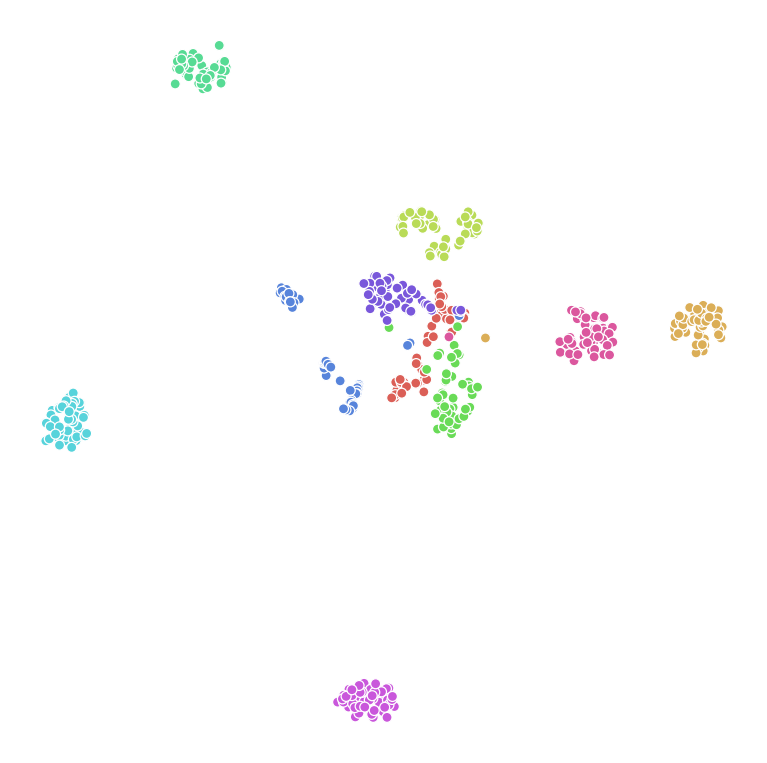
\includegraphics[width=0.9\textwidth]{figs/tsne-clmr.png}
    \caption{$t$-SNE manifold visualisation from audio representations learned by a converged CLMR model of a subset of 10 tracks with each 60 segments.
Every color represents a separate track.}
    \label{fig:tsne_manifold}
\end{figure}

\begin{figure*}[h]
    \centering
    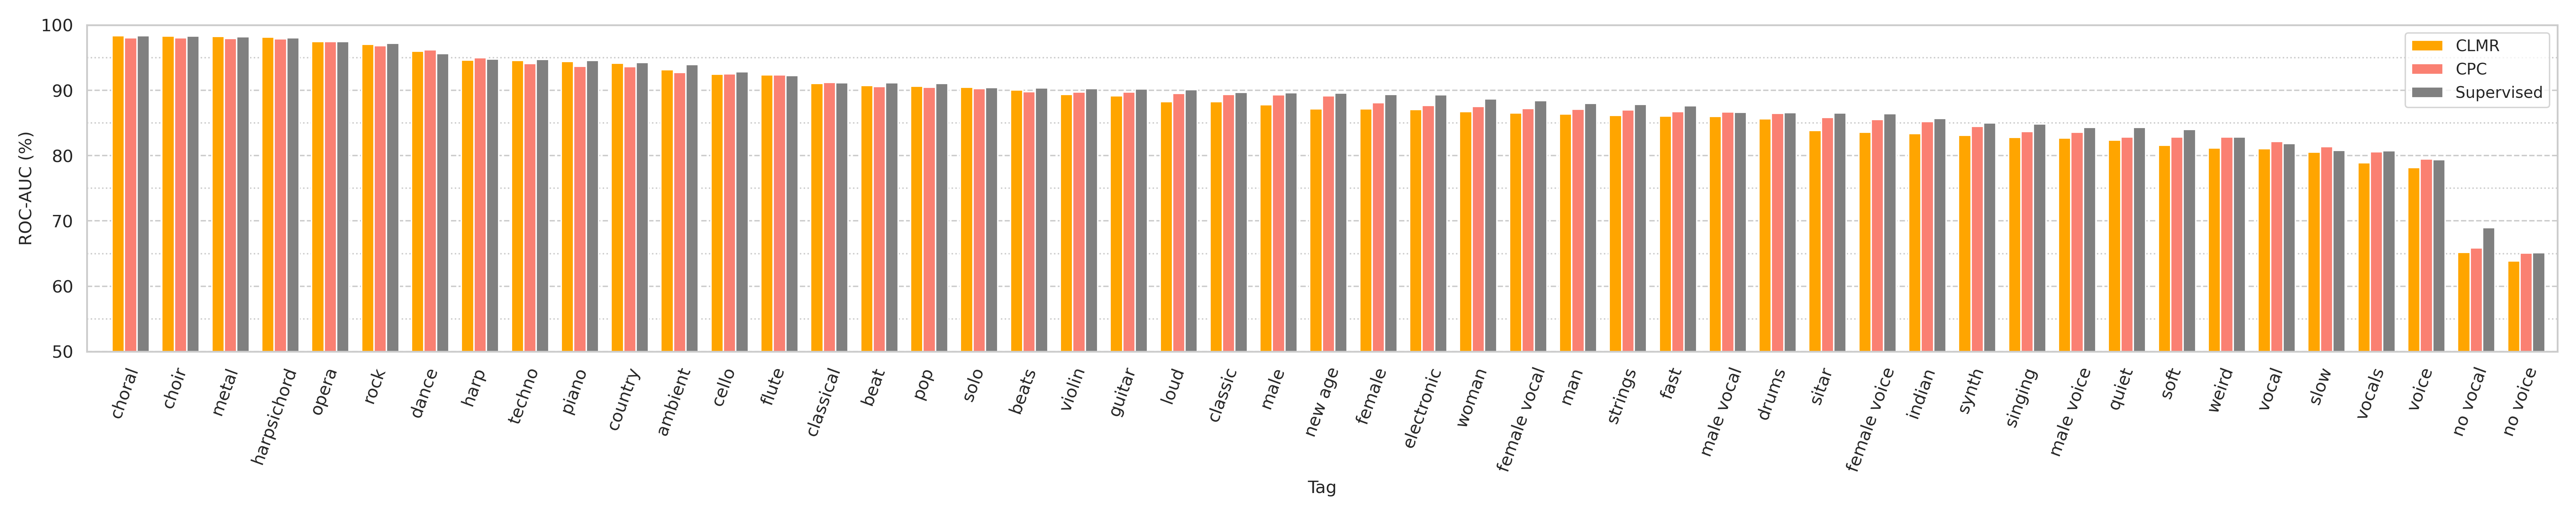
\includegraphics[width=\textwidth]{figs/tag_retrieval.png}
    \caption{Tag-wise ROC-AUC scores for the top-50 tags in the MagnaTagATune dataset, reported for linear, logistic regression classifiers trained on representations of self-supervised models CLMR and CPC, and compared to a fully supervised, end-to-end SampleCNN model.}
    \label{fig:tag_scores}
\end{figure*}


\section{Data Augmentations}\label{sec:data_augmentations}
The CLMR model relies on a pipeline of strong data augmentations to facilitate the learning of representations that are more robust and allow for better generalisation in the downstream task.
In Figure \ref{fig:transformation_study}, we show the PR-AUC linear evaluation score that is achieved when taking a random slice of audio (`random cropping') and performing one additional, individual augmentation.
While all datasets contain songs of variable length, we always sample a random slice of audio of the same size before applying other augmentations.
Since we always have to take a random slice, it makes it harder to assess the individual contribution of each augmentation to the downstream task performance.
We therefore consider an asymmetric data transformation setting: we only apply the augmentation pipeline to one branch of the framework, while we settle with an identity function for the other branch (i.e., $t(x_j) = x_j$) \cite{chen_simple_2020}. The transformations on the augmentation branch are applied with probability $p_t=1$, i.e., the transformation is always applied.

When only taking a random slice of audio (i.e., a `crop'), we achieve a PR-AUC score of 30.5.
Most augmentations show a similar increase in performance of ±31.5, while adding gain or delay does not impact performance as much.
Adding a filter to the pipeline increases the downstream performance significantly.

\begin{figure*}[h]
    \centering
    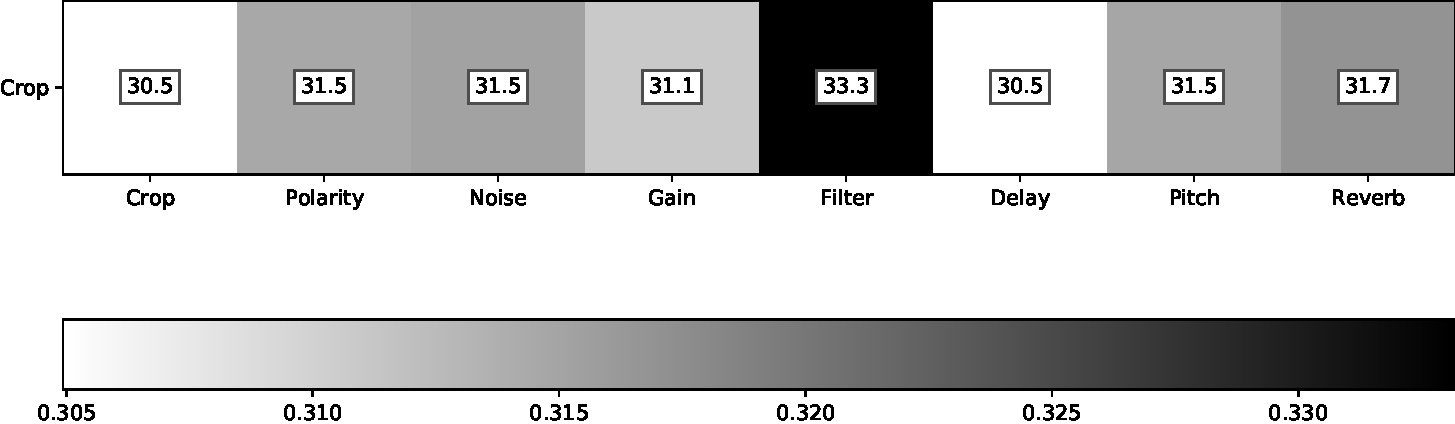
\includegraphics[width=\columnwidth]{figs/transformation_study.pdf}
    \caption{The achieved $\mathrm{PR-AUC}_{\mathrm{TAG}}$ score using a random crop together with one other transformation}
    \label{fig:transformation_study}
\end{figure*}

Besides evaluating the individual contribution of each augmentation with a probability of $p_t = 1$, we also vary this probability: $p_t \in \{ 0, 0.4, 0.8 \}$.
This is done to assess the optimal amount of augmentation to each example, i.e., the contrastive learning task should not be too hard, neither too simple, for learning effective representations in the downstream music classification task.
The linear evaluation PR-AUC score is shown for each augmentation under a different probability $p_t$ in Figure \ref{fig:transformation_probabilities}. For the Polarity and Filter transformations, performing them more often with a probability of $p_t = 0.8$ is beneficial. For the Delay, Pitch and Reverb transformations, a transformation probability of $p_t = 0.4$ works better than performing them more aggressively.

\begin{figure}[h]
    \centering
    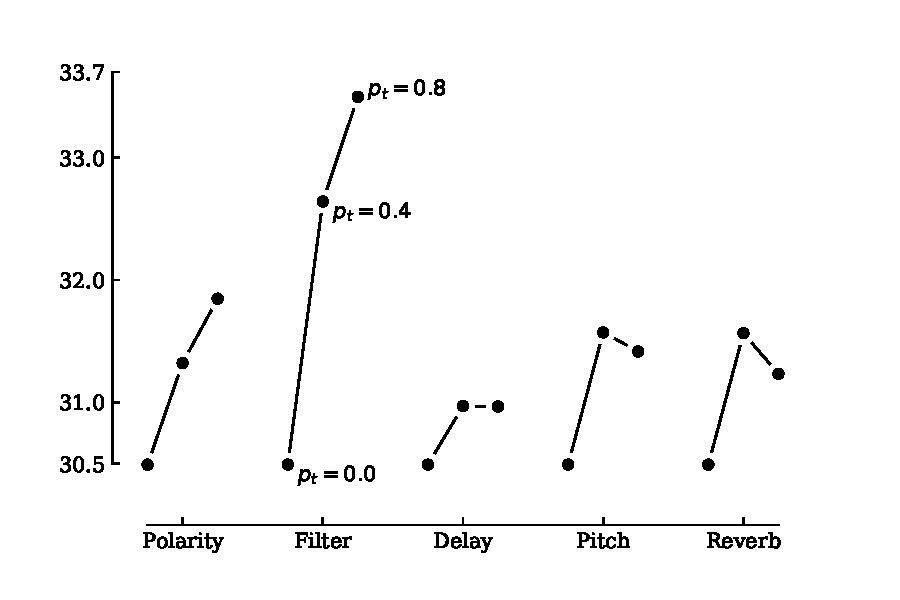
\includegraphics[width=\columnwidth]{figs/transformation_probabilities.pdf}
    \caption[-5cm]{$\mathrm{PR-AUC}_{\mathrm{TAG}}$ scores for transformations under different, consecutive probabilities $p \in \{ 0.0, 0.4, 0.8 \}$}
    \label{fig:transformation_probabilities}
\end{figure}


\section{Efficient Classification Experiments}
When training on a specific task like music classification, only a limited amount of labeled data may be available. To test the efficient classification capability of the CLMR model, we fine-tune the linear classifier on 1\% of the labels in the dataset and report its performance. During the task-agnostic, self-supervised pre-training phase, 100\% of the data is used. As outlined previously, the representations that are learned during this phase are subsequently used during linear evaluation.

Figure \ref{fig:perc_train_data_magnatagatune} and \ref{fig:perc_train_data_msd} show the PR-AUC scores obtained when increasing the amount of labels available during fine-tuning.
For both datasets, fine-tuning using just $1\%$ of the labels yields a large performance difference compared to training in a fully supervised manner, while using the same amount of labels.

\begin{figure}[h]
    \centering
    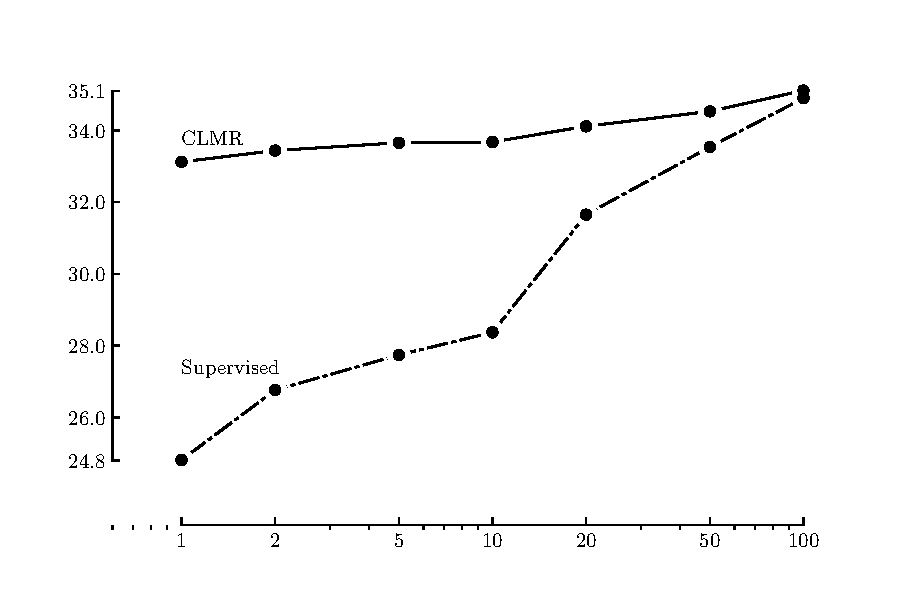
\includegraphics[width=\columnwidth]{figs/perc_train_data_magnatagatune.pdf}
    \caption{Percentage of labels used for training vs. the achieved $\mathrm{PR-AUC}_{\mathrm{TAG}}$ score on the MagnaTagATune dataset}
    \label{fig:perc_train_data_magnatagatune}
\end{figure}


Using 100$\times$ fewer labels, CLMR scores 33.1\% PR-AUC compared to 24.8\% PR-AUC obtained with an equivalent, end-to-end trained supervised model.
Pre-training using a self-supervised objective without labels therefore substantially improves efficient classification: only $1\%$ of the labels are required while maintaining a similar performance.

For the Million Song Dataset, a fully supervised end-to-end trained model exceeds CLMR at $10\%$ of the labels, which are 24,190 unique songs in total. Beyond this amount of music, CLMR is unable to perform in a trend similar to the supervised model.

\begin{figure}[h]
    \centering
    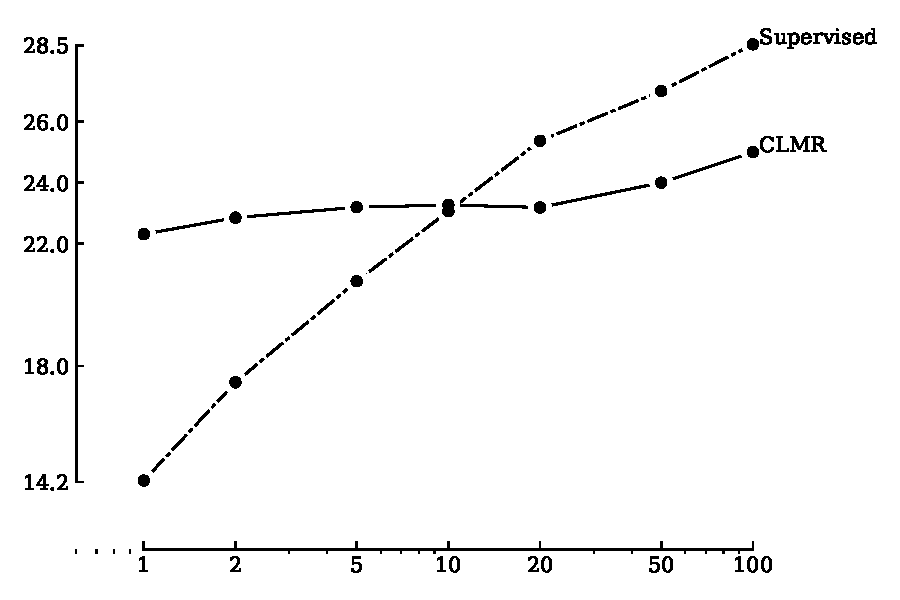
\includegraphics[width=\columnwidth]{figs/perc_train_data_msd.pdf}
    \caption{Percentage of labels used for training vs. the achieved $\mathrm{PR-AUC}_{\mathrm{TAG}}$ score on the Million Song Dataset.}
    \label{fig:perc_train_data_msd}
\end{figure}



\section{Transfer Learning Experiments}
The results of the transfer learning experiments are shown in Table \ref{tab:magnatagatune_results}.
Both CPC and CLMR show the ability to learn effective representations from datasets different from the evaluation dataset without ground truth, and even exceed accuracy scores of previous, supervised end-to-end systems on raw audio \cite{dieleman2014end}.
Moreover, both models demonstrate the ability to learn useful representations on the much smaller GTZAN and Billboard datasets.
The CLMR model performs better when it is pre-trained on larger datasets, which is expected as it heavily relies on the number of unique, independent examples that make the contrastive learning task harder, resulting in more robust representations.
When pre-training on smaller datasets, the autoregressive modelling in CPC can find more useful representations for downstream tasks.
%contribute to more useful representations for downstream tasks.

\begin{table}[h]
    \centering
    \begin{tabular}{@{}lllcc@{}}\toprule
        Model & Train Dataset & Eval.
        Dataset &  ROC-AUC & PR-AUC \\ \midrule
        CLMR & MSD & MTAT &  86.57 & 32.04 \\
        CPC & FMA & MTAT & 86.34 (87.79) & 30.71 (32.47) \\
        CLMR & FMA & MTAT & 86.22 (86.63) & 30.58 (31.22) \\
        CPC & Billboard & MTAT & 85.78 (86.25) & 29.68 (30.15) \\
        CPC & GTZAN & MTAT & 83.44 (86.06) & 26.88 (29.72) \\
        CLMR & Billboard & MTAT & 82.73 (84.22) & 26.86 (27.82) \\
        CLMR & GTZAN & MTAT & 81.88 (85.43) & 26.18 (29.49) \\
        \bottomrule
    \end{tabular}
    \caption{Performance of the self-supervised models when pre-trained on datasets different from the evaluation dataset, again using a linear classifier to evaluate.}
    \label{tab:magnatagatune_results}
\end{table}

\newpage

\section{Additional Experiments}\label{sec:additional_experiments}
\subsection{Mini-batch Size}\label{sec:exp_mini_batch_size}
The complexity of the pretext task increases with larger mini-batch sizes. To reiterate: in our pretext task, it is harder for the the model to infer the positive pair when increasing the pool of negative examples.
To further study the quality of the repesentations for the downstream task performance, given the increase of complexity of the pretext task, we experimented with varying mini-batch sizes while keeping all other parameters the same.

We use the default sample rate of 22\,050~Hz, the $3^9$ SampleCNN encoder network, train all experiments for 3\,000 epochs and set the transformation probabilities to their optimal value, as demonstrated in Section \ref{sec:data_augmentations}. All models with varying mini-batch sizes are trained from scratch and evaluated using the linear evaluation procudure outlined in Section \ref{sec:evaluation}.

While our smallest model already shows competitive performance compared to fully supervised models, the performance increased when using 96 examples per mini-batch. Our largest model did not perform as expected, and scores consistently lower than our middle-sized model. This may be attributed to a sub-optimal configuration of the optimiser, i.e., the LARS optimiser that is used for larger mini-batch sizes. Another theory, is that the task of inferring the positive pair of 2.6 second long audio fragments, in a pool of 912 negative samples, may require even longer training, or is simply too hard. The results of this experiment are shown in Table \ref{tab:mini_batch_ablation}.


\begin{table*}
    \centering
    \begin{tabular}{lllll}\toprule
    Mini-batch Size & $\text{ROC-AUC}_{\text{TAG}}$ & $\text{PR-AUC}_{\text{TAG}}$ & $\text{ROC-AUC}_{\text{CLIP}}$ & $\text{PR-AUC}_{\text{CLIP}}$ \\\midrule
    456 & 88.13 & 34.87 & 92.96 & 68.90 \\
    96 & 88.49 & 35.11 & 93.07 & 69.20 \\
    48 & 87.91 & 34.56 & 92.88 & 68.75 \\\bottomrule
    \end{tabular}
    \caption[][24pt]{Effect of the mini-batch size used during self-supervised training on the music classification task performance.}
    \label{tab:mini_batch_ablation}
\end{table*}


\subsection{Training Duration}
Contrastive learning techniques have shown to benefit from longer training compared to their supervised equivalent \cite{chen_simple_2020}. While larger mini-batch sizes increase the number of negative examples the model can `see' simultaneously, training for a longer time increases the number of negative examples the model sees overall. We vary the number of epochs we train the model for, while we keep all other parameters constant, i.e., identically to those described in Section \ref{sec:exp_mini_batch_size}. The mini-batch size is set to 96 and all models are again trained from scratch and evaluated using the linear evaluation procedure.

Increasing the self-supervised training duration improves the downstream task performance. Our best results are obtained when training the CLMR model for 10\,000 epochs. When training the logistic, linear regression classifier on the learned representations, it perfroms better than a fully, end-to-end trained supervised model. The results of this experiment are shown in Table \ref{tab:epoch_ablation}.


\begin{table*}
    \centering
    \begin{tabular}{lllll}\toprule
    Epochs & $\text{ROC-AUC}_{\text{TAG}}$ & $\text{PR-AUC}_{\text{TAG}}$ & $\text{ROC-AUC}_{\text{CLIP}}$ & $\text{PR-AUC}_{\text{CLIP}}$ \\\midrule
    10\,000 & 88.47 (89.25) & 35.37 (35.89) & 93.16 (93.48) & 69.32 (70.03) \\
    3\,000 & 88.49 (88.94) & 35.11 (35.46) & 93.07 (93.27) & 69.20 (69.74) \\
    1\,000 & 88.31 (88.64) & 34.40 (34.86) & 92.89 (93.08) & 68.59 (69.15) \\\bottomrule
    \end{tabular}
    \caption[][24pt]{Effect of the self-supervised training duration on the music classification task performance.}
    \label{tab:epoch_ablation}
\end{table*}




\subsection{Sample Rates}    
When re-sampling the audio to 8\,000~Hz and 16\,000~Hz respectively, there is a marginal penalty to the final scores for the self-supervised models, which is in line with previous work \cite{lee2018samplecnn}. In Table \ref{tab:sample_rate_ablation}, we show all linear evaluation scores when no additional transformations are performed (i.e., only random cropping) to isolate the contribution of each individual sample rate.


\begin{table*}
    \centering
        \begin{tabular}{lllll}\toprule
        Sample rate & $\text{ROC-AUC}_{\text{TAG}}$ & $\text{PR-AUC}_{\text{TAG}}$ & $\text{ROC-AUC}_{\text{CLIP}}$ & $\text{PR-AUC}_{\text{CLIP}}$ \\\midrule
        8\,000 & 84.78 & 29.77 & 90.60 & 62.94 \\
        16\,000 & 85.46 & 30.42 & 90.97 & 64.08 \\
        22\,050 & 85.82 & 30.49 & 91.25 & 64.78 \\                       
        \bottomrule
        \end{tabular}
    \caption[][24pt]{Effect of the sample rate on tag prediction performance.}
    \label{tab:sample_rate_ablation}
\end{table*}


% \subsection{Projector Network}
% A non-linear projector network positively impacts the performance of the model.
% Adding only one extra hidden layer to the classifier increases the results by $4\%$, making the gap between supervised end-to-end baselines even smaller.
% It is clear from these results that useful representations can be learned from high-dimensional signals of raw audio even without access to ground truth labels.

\subsection{Temperature}
The temperature parameter $\tau$ in the NT-Xent loss function (Equation \ref{eq:loss_function}) controls the penalty given to the negative samples. The experiments in Table \ref{tab:temperature_ablation} are run using a mini-batch size of 96, which is a smaller mini-batch size than those used in the original SimCLR paper (i.e., $\leq 4096$ samples per mini-batch) \cite{chen_simple_2020}. Consequently, the performance difference is marginal. Again, no additional transformations except random cropping are applied in this experiment to isolate the contribution of this temperature parameter.

\begin{table*}
    \centering
    \begin{tabular}{lllll}\toprule
    Temperature & $\text{ROC-AUC}_{\text{TAG}}$ & $\text{PR-AUC}_{\text{TAG}}$ & $\text{ROC-AUC}_{\text{CLIP}}$ & $\text{PR-AUC}_{\text{CLIP}}$ \\\midrule
    0.1  & 85.82  & 30.33 & 91.18 & 64.10 \\
    0.3 & 85.58 & 30.35 & 91.21  & 64.38 \\
    0.5 & 85.82 & 30.49 & 91.25 & 64.78 \\                       
    \bottomrule
    \end{tabular}
    \caption[][24pt]{Ablation study of the temperature parameter in the NT-Xent loss function.}
    \label{tab:temperature_ablation}
\end{table*}


\section*{Summary}
In this chapter, we presented the results of this thesis. We showed that CLMR learns effective representations from raw signals of musical audio. Despite self-supervised pre-training and fine-tuning a linear classifier on the representations, we achieve strong performance on the downstream music classification task. CLMR outperforms the current state-of-the-art waveform-based model on the MagnaTagATune dataset, but it requires longer training to show comparable results on the Million Song Dataset.

We studied the contribution of seven different data augmentations, of which five were studied with altering transformation probabilities, to the robustness of the learned representations. In line with previous research on self-supervised learning, we demonstrated that strong data augmentations during pre-training benefit the downstream task performance. We also showed that too strong augmentations can negatively impact the usability of the representations.

It is common in MIR to have limited labeled data available for training a neural network. Therefore, we tested the efficient classification capability of the CLMR model. We fine-tuned the linear classifier on only 1\% of the labels in the dataset, using representations learned during the self-supervised pre-training phase on 100\% of the data. The linear classifier still achieved 33.1\% PR-AUC, compared to 24.8\% PR-AUC with a fully supervised end-to-end model, despite using 100$\times$ fewer labels.

Lastly, we showed that the learned representations are transferable across different musical corpora. When pre-training CLMR on a large, out-of-domain music dataset, and linearly evaluating the representations on another music dataset, the cost is a relatively small performance margin.